\mySection{13.A Appendix: Some Discussions and Extensions}
%-------------- start slide -------------------------------%{{{
\begin{frame}{\S\: 13.A Appendix: Some Discussions and Extensions }

\centering
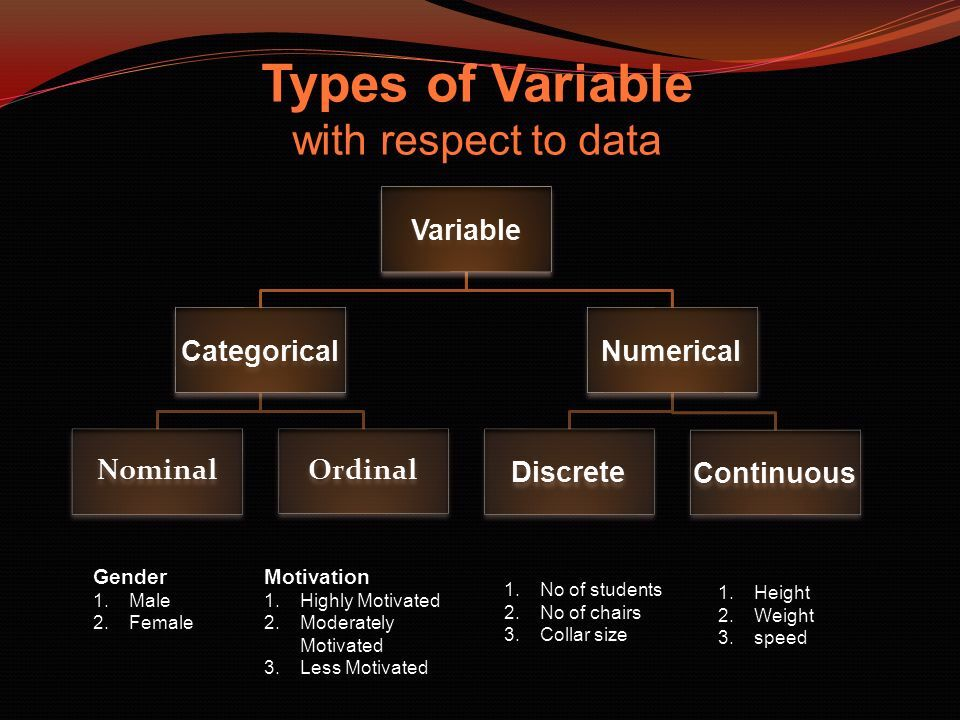
\includegraphics[scale=0.4]{Types+of+Variable+with+respect+to+data-neg.jpg}
\end{frame}
%-------------- end slide -------------------------------%}}}
%-------------- start slide -------------------------------%{{{
\begin{frame}[fragile]
\centering
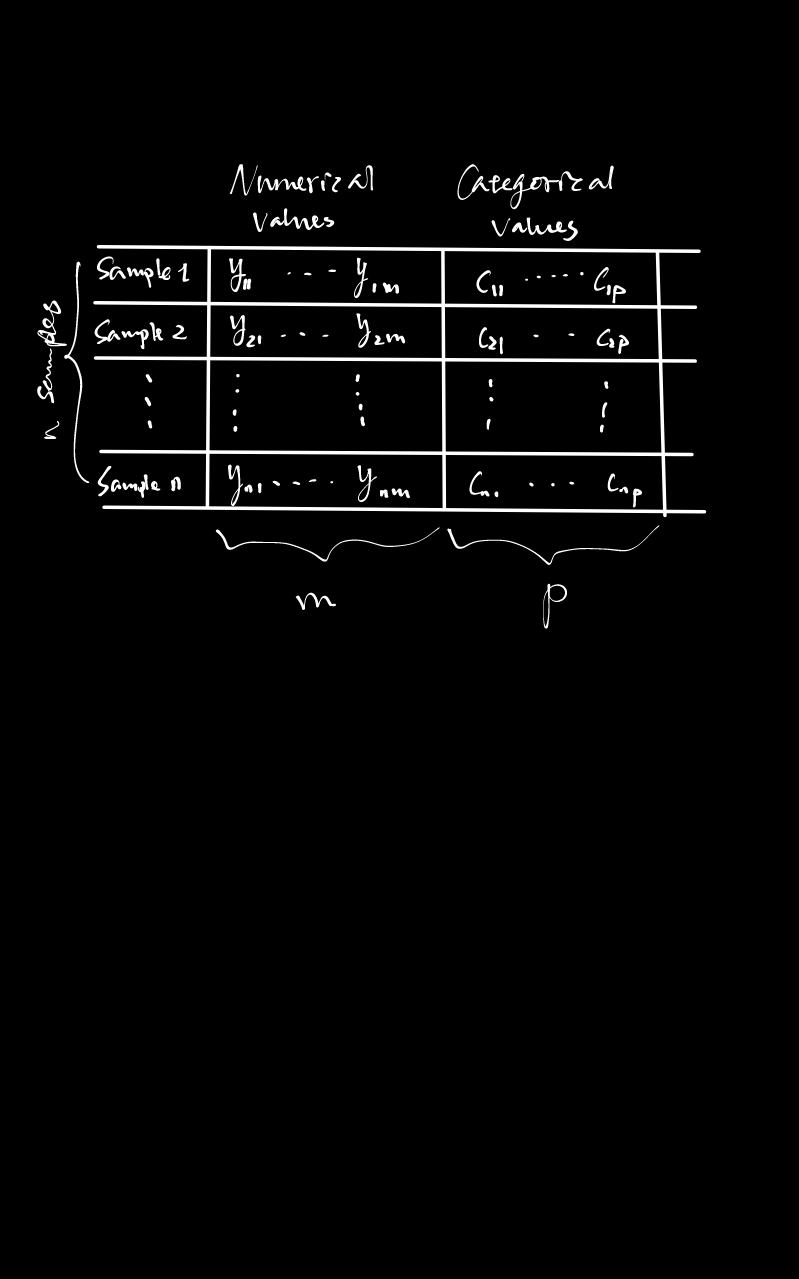
\includegraphics[scale=0.35]{Features2-neg.png}
\end{frame}
%-------------- end slide -------------------------------%}}}
%-------------- start slide -------------------------------%{{{
\begin{frame}[fragile]
\centering
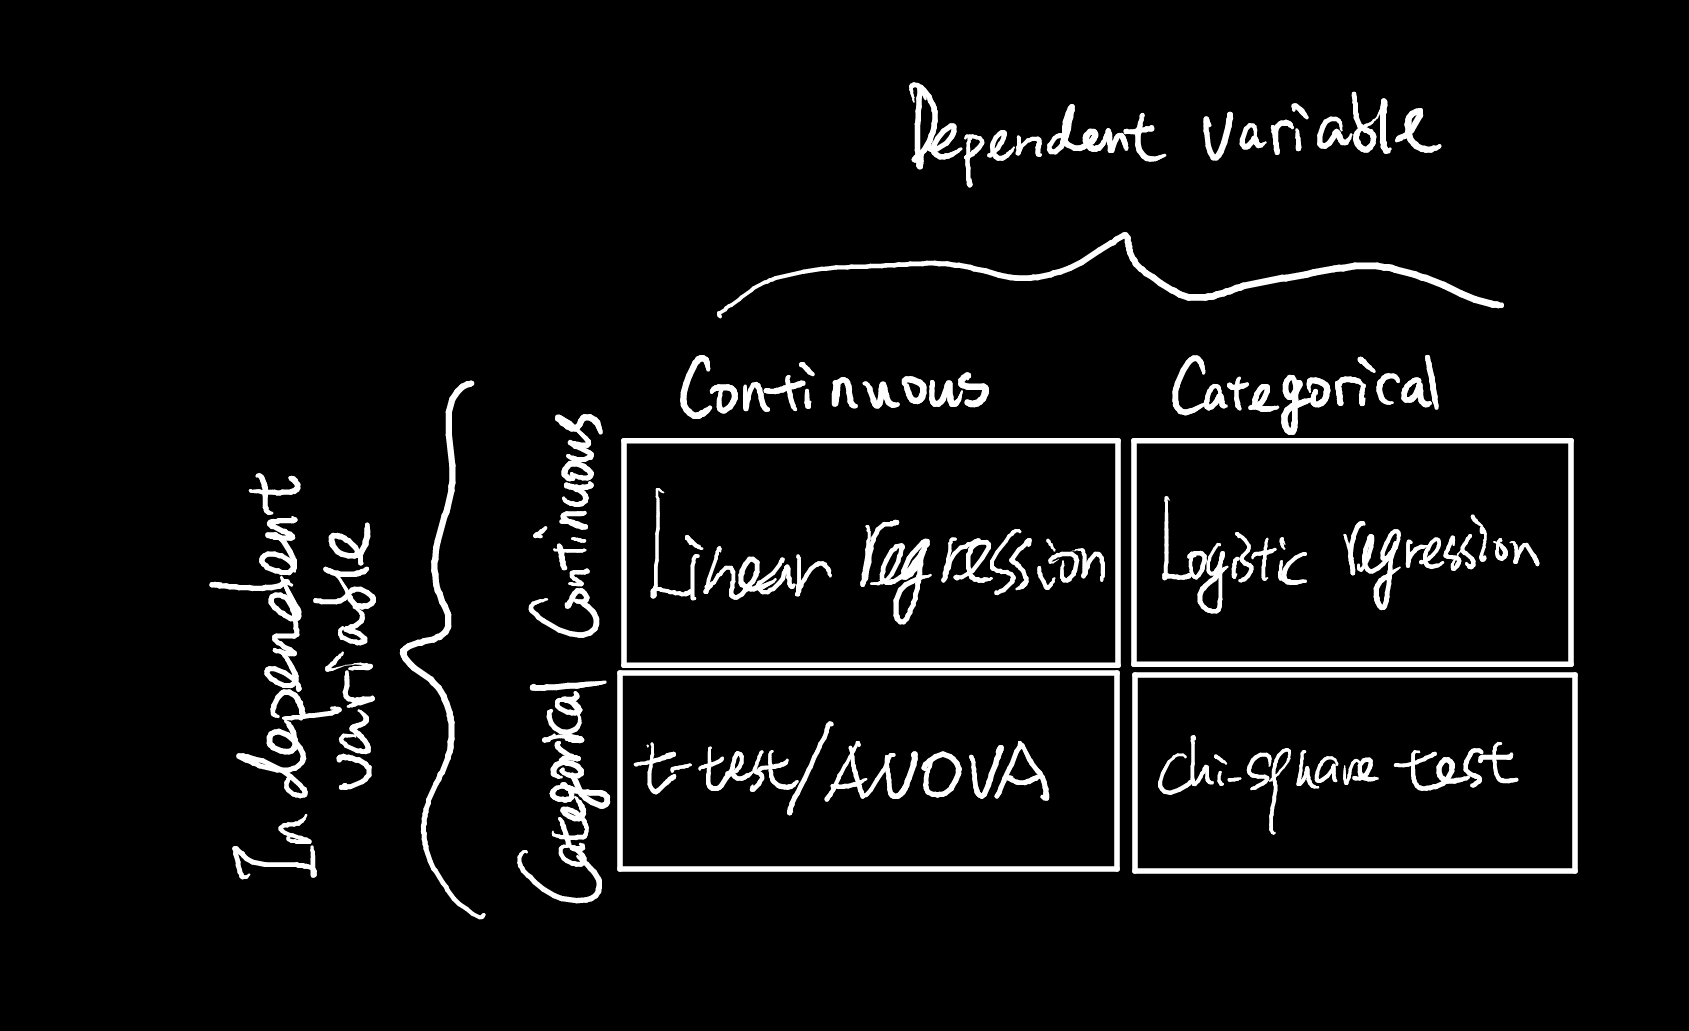
\includegraphics[scale=0.18]{Methods5-neg.png}
\end{frame}
%-------------- end slide -------------------------------%}}}
%-------------- start slide -------------------------------%{{{
\begin{frame}[fragile]

\begin{enumerate}
\item[] Indep. \quad v.s. \quad Dependent
\item Categorical v.s. Continuous
\item[]
\begin{minipage}{0.7\textwidth}
\begin{enumerate}
\item $p=1$, $m=1$,\hfill One-way ANOVA
\item $p=2$, $m=1$,\hfill Two-way ANOVA
\item $p\ge 3$, $m=1$,\hfill $p$-way ANOVA
\\[2em]
\item $p=1$, $m\ge 2$,\hfill One-way MANOVA\footnote{MANOVA refers to the multivariate analysis of variance\\
\hspace{2em} ANOVA refers to the univariate analysis of variance.}
\item $p=2$, $m\ge 2$,\hfill Two-way MANOVA
\item $p\ge 3$, $m\ge 2$,\hfill $p$-way ANOVA
\end{enumerate}
\end{minipage}
\vfill
\item Continuous v.s. Continuous
\item[]
\begin{minipage}{0.7\textwidth}
\begin{enumerate}
\item $m_{ind}=1$, $m_{dep}=1$,\hfill Simple linear regression
\item $m_{ind}\ge 2$ \hfill Multiple linear regression
\item $m_{dep}\ge 2$ \hfill Multivariate linear regression
\end{enumerate}
\end{minipage}
\end{enumerate}
\end{frame}
%-------------- end slide -------------------------------%}}}
%-------------- start slide -------------------------------%{{{
\begin{frame}[fragile]
\begin{itemize}
\item[E.g.] One example for MANOVA\footnote{\url{http://www.sthda.com/english/wiki/manova-test-in-r-multivariate-analysis-of-variance}}.
\vfill
\begin{center}
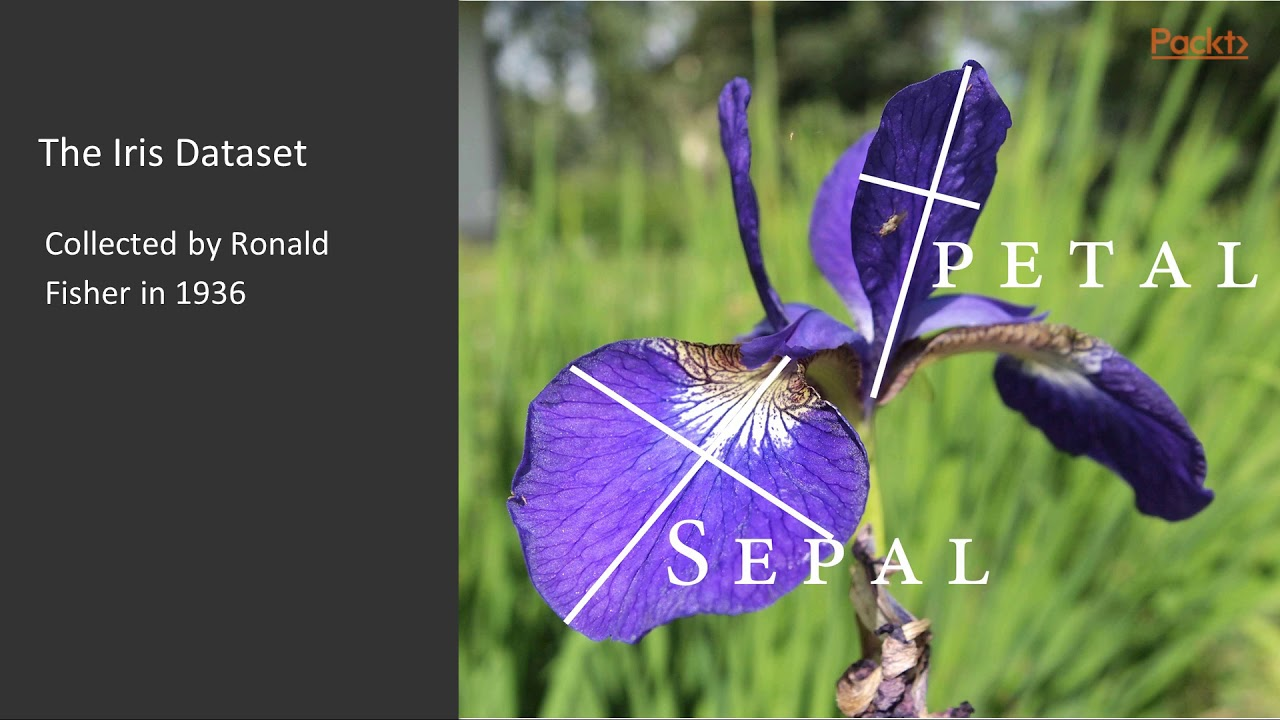
\includegraphics[scale=0.15]{Iris_Dataset_Fisher.jpg}
\end{center}
\end{itemize}
\end{frame}
%-------------- end slide -------------------------------%}}}
%-------------- start slide -------------------------------%{{{
\begin{frame}[fragile]
\begin{center}
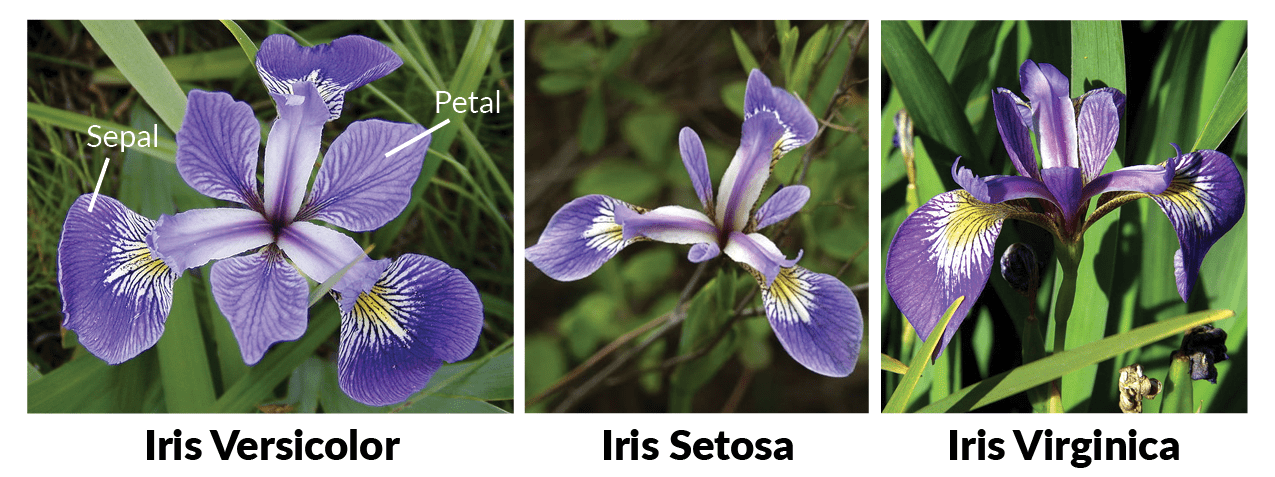
\includegraphics[scale=0.25]{Iris_Dataset_Fisher2.png}
\end{center}
\end{frame}
%-------------- end slide -------------------------------%}}}
%-------------- start slide -------------------------------%{{{
\begin{frame}[fragile]
\begin{center}
\begin{minipage}{0.8\textwidth}
\begin{lstlisting}
> library(datasets)
> data(iris)
> summary(iris)
  Sepal.Length    Sepal.Width     Petal.Length    Petal.Width          Species
 Min.   :4.300   Min.   :2.000   Min.   :1.000   Min.   :0.100   setosa    :50
 1st Qu.:5.100   1st Qu.:2.800   1st Qu.:1.600   1st Qu.:0.300   versicolor:50
 Median :5.800   Median :3.000   Median :4.350   Median :1.300   virginica :50
 Mean   :5.843   Mean   :3.057   Mean   :3.758   Mean   :1.199
 3rd Qu.:6.400   3rd Qu.:3.300   3rd Qu.:5.100   3rd Qu.:1.800
 Max.   :7.900   Max.   :4.400   Max.   :6.900   Max.   :2.500
> my_data <- iris
> my_data
    Sepal.Length Sepal.Width Petal.Length Petal.Width    Species
1            5.1         3.5          1.4         0.2     setosa
2            4.9         3.0          1.4         0.2     setosa
3            4.7         3.2          1.3         0.2     setosa
4            4.6         3.1          1.5         0.2     setosa
5            5.0         3.6          1.4         0.2     setosa
6            5.4         3.9          1.7         0.4     setosa
7            4.6         3.4          1.4         0.3     setosa
8            5.0         3.4          1.5         0.2     setosa
9            4.4         2.9          1.4         0.2     setosa
10           4.9         3.1          1.5         0.1     setosa
\end{lstlisting}
\end{minipage}
\end{center}
\end{frame}
%-------------- end slide -------------------------------%}}}
%-------------- start slide -------------------------------%{{{
\begin{frame}[fragile]
\begin{center}
\begin{minipage}{0.9\textwidth}
\begin{lstlisting}
> # Compute MAOVA test now
> res.man <- manova(cbind(Sepal.Length, Petal.Length) ~ Species, data = iris)
> summary(res.man)
           Df Pillai approx F num Df den Df    Pr(>F)
Species     2 0.9885   71.829      4    294 < 2.2e-16 ***
Residuals 147
---
Signif. codes:  0 '***' 0.001 '**' 0.01 '*' 0.05 '.' 0.1 ' ' 1
> # Look to see which differ
> summary.aov(res.man)
 Response Sepal.Length :
             Df Sum Sq Mean Sq F value    Pr(>F)
Species       2 63.212  31.606  119.26 < 2.2e-16 ***
Residuals   147 38.956   0.265
---
Signif. codes:  0 '***' 0.001 '**' 0.01 '*' 0.05 '.' 0.1 ' ' 1

 Response Petal.Length :
             Df Sum Sq Mean Sq F value    Pr(>F)
Species       2 437.10 218.551  1180.2 < 2.2e-16 ***
Residuals   147  27.22   0.185
---
Signif. codes:  0 '***' 0.001 '**' 0.01 '*' 0.05 '.' 0.1 ' ' 1:w
\end{lstlisting}
\end{minipage}
\end{center}
\vfill

\begin{enumerate}
\item[Concl.:] Two variables are highly significantly different among species.
\end{enumerate}
\end{frame}
%-------------- end slide -------------------------------%}}}
